\chapter{Introduction}
\label{chapter:introduction}

\section{Overview}

The context of the rendering application always dictate the constraints
applied to the methods and algorithms used by the software for the image generation.
Modern approaches to realictic rendering could be roughly divided into distinct
groups:
physically based rendering (light simulation approach) and plausible rendering
(phenomenological approach).

Physically based rendering tries to simulate interaction of the light and matter
taking into account the laws of physics and our theoretical knowlage about the
natue.

Plausible rendering, on the other hand, is intended to mimic optical effects
observed by the human eye or captured by camera accounting the audience
preception.

While Monte Carlo methods of the light simulation are usually perceived as
physically based methods. Sometimes they are also used for relatively fast way
to achive desired plausible optical effects.

\section{Scope}
In this paper I study Monte Carlo rendering of the subsurface scattering
materials, both in the context of light simulation and plausible rendering.
The main interest is in the correctness of the methods and the
consistency of the results between them. With the discussion of the optimisation
techniques applicable in certain scenarios.

I focus on the methods of the rendering of highly scattering isotropic materials
which usually appear as optically thick objects.

These are examples of the materials which, in most cases, meet that condition.
\begin{itemize}
    \item Non-organic
    \begin{itemize}
        \item Marble (polished, rough, dusty)
        \item Plastics or waxes
        \item Snow
        \item Thin sheets (paper, foilage, cloth)
        \item Non photoreal (Cartoon style and stylisation)
    \end{itemize}
    \item Organics
    \begin{itemize}
    \item Optically thick liquids (milk, some kinds of juice)
        \item Skin (sweaty, dry, makeup)
        \item Food (cheese, meat, bread, some kinds of fruits)
    \end{itemize}
\end{itemize}
These are examples of materials out of scope:
\begin{itemize}
    \item Highly transparent liquids (dirty/dusty water, ocean water, wine)
    \item Fluids (air, fog, dust)
\end{itemize}
I consider only isotropic media which are modeled by means of geometric
polygonal meshes. The constraint of the closed shape in not applicable to all
the methods discussed and will be discussed later.

I do not consider spectral scattering. Only monochromatic light is simulated.
There are papers describing the process of combined rendering of RGB with
corresponding importance sampling. To add.

Why not to use point cloud based approach:
\begin{itemize}
    \item{Ease of use for the user. Don't want to introduce a lot of control
    parameters which often require the end user to learn the details of the
    underlying algorithms}
    \item{Undesired preprocessing step. Unfriendly to progressive rendering}
    \item{Density of the generated point cloud (or other stucture) limits the
    scope of the available parameters. It restrics the effective width of the
    SSS by minimal distanse between points, for example. Point density $\approx$
    mean free path}
    \item{Possible flickering artifacts during animation}
    \item{Additional memory requirements}
    \item{Workflow complications for storing data additional data}
\end{itemize}

Other things to consiger while choosing method:
\begin{itemize}
  \item Lighting restrictions \emph{Analytic light} sources and \emph{area lights and IBL} friendly
  \item Multiple object friendly
  \item Parametrization Artist friendly or physically correct
  \item Homogeneous or inhomogeneous
  \item Performance. Is it suitable for real time application?
\end{itemize}

\section{Unidirectional path tracing}
Unidirectional path tracing \gls{UDPT} or simply path tracing is one of the
fundamental methods of Monte Carlo light integration in computer graphics.

In practice, almost always contains Russian Roulette otimization. Detailed
description is in section \ref{subsection:rr}. It is a robust technique, leaving
the integrator unbiased. But may has some non obvious numerical problems
especially while being used in scenarious like volumetric rendering (see
chapter \ref{section:numerical})

\ldots

A typical disadvantage of the classic \gls{UDPT} is the high variance and
subsecuently strong noise component in the rendered images of the scenes with 
highly non-uniform incoming illumination.
In practice, these scenes contain small but intensive emitters or direct sun
light in the image-based lighting scenes. The extreme worst case is the
prensence of the analytic light sources: point lights with zero area or
directional lights, having virtually infinite distance to the shaded locaten.

\subsection{UDPT with direct light sampling}
Although \gls{UDPT} is proved to be a robust unbiased estimator, it has some
limitations.
\begin{figure}
    \centering
    \begin{subfigure}{0.45\textwidth}
        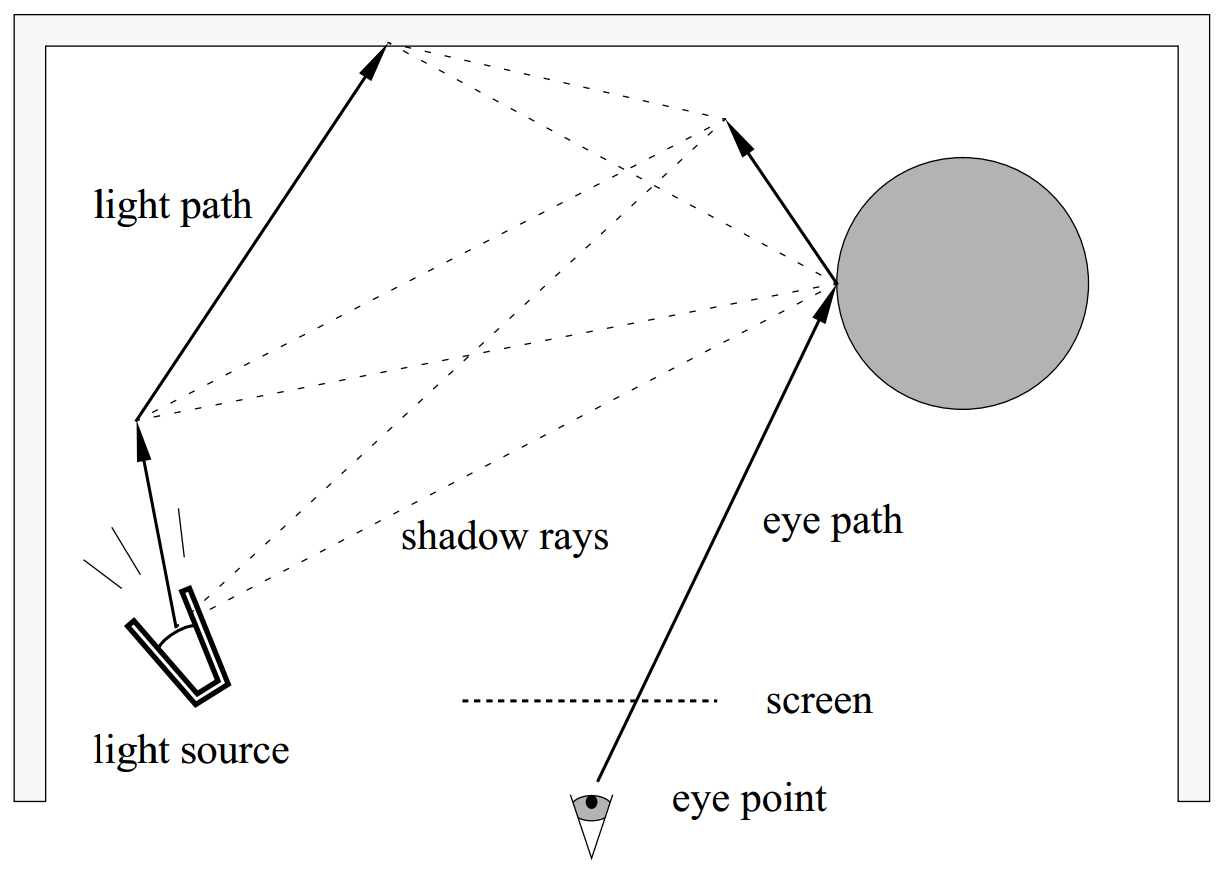
\includegraphics[width=\textwidth]{imgs/schemes/generalized_BDPT_lafortune}
        \caption{general}
        \label{fig:bdptgeneral}
    \end{subfigure}
    \begin{subfigure}{0.45\textwidth}
        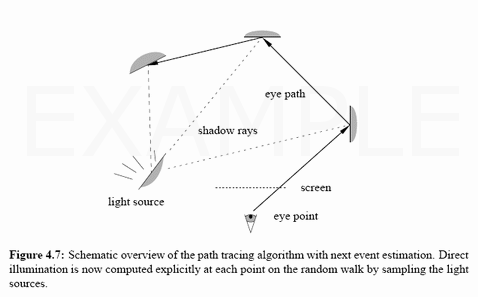
\includegraphics[width=\textwidth]{imgs/schemes/PT2_resize}
        \caption{special}
        \label{fig:udpt_ptdl}
    \end{subfigure}

    \caption{BDPT temp illustrations}
    \label{fig:bdpt}
\end{figure}


Next Event Estimation (\gls{NEE}) is one of the common methods of reducing a
variance of the path tracing. The main idea of the \gls{NEE} is to estimate
\textit{direct illumination} by sampling the light source directly at each step
of the path tracing. Then, the shadow test ray is needed to ensure that the
current light sampling position in visible by the surface.

\gls{NEE} can also be considered as the special case of the general
Bidirectional Path Tracing algorithm \gls{BDPT} \cite{Veach:94:BDPT}.
\ref{fig:bdpt} Using the vocabulary of the original paper, NEE algorithm is
\textit{(m,2)-method}. with the length of light path equals 2 and length of the eye path $m\geq3$ is defined by
the \gls{UDPT} settings.

\subsection{Volumetric Path Tracing}
Path tracing with light scattering inside the media
Dwivedi sampling scheme

\subsection{Volumetric path tracing with Next Event Estimation}
The idea of direct light sampling can be applied to the volumetric path tracing
as well.
The generalized theory of \gls{BDPT} in participating media was first described
by Lafortune ans Willems in \cite{Lafortune:1996:RPM:275458.275468}. 

\ldots

Preforming the direct light estimation from inside the media with the refractive
boundry proved to be a non-trivial task.
Due to the refraction on the boundary between materials with different index of
refraction (\gls{IOR}), the light from the emitter to the scattering point never
travels by a straight light. Except the casse of the normal incident rays. To
satisfy the Fermat's principle
\footnote{Fermat's principle or the principle of least time states that the path taken between two points by a ray of light is the path that can be traversed in the least time}
we have to construct the path with the middle point somewhere on the boundry.

To my knowledge, there are no robust and fast enough methods for solving this
complication in general way. Although, there are considerable iterative
approaches described in the literature during last years
\cite{holzschuch:hal-01083246}, \cite{10.1111:cgf.12681}, \cite{Koerner2016}.

In this work I have decided to consider the situation when the bounary
refraction can be neglected. In the other words, the materials with \gls{IOR}=1.
It leads to the approximation of the direct light path from inside the media to the light source as a straigt line. This assumption certainly
introduces an error in the simulation. But the error is significant only for
optically low dense materials. Light propagation in highly scattering media, in
contrast, is charachterized by many scattering events. Which makes the direction
of the first ray less important for the future light simulation.

\section{Intuition behind Diffusion approximation and BSSRDF formulation}

\subsection{Analogy to BRDF approximation}
Formulate scattering in media in analogy to local surface reflectance (BRDF)

\subsection{Single scattering and Multiple scattering}
Decompose into single- and multiscattering terms

\subsection{Double scattering paper}
\cite{Donner:2009:EBM} model is the most accurate to date (2013), but it has a
high memory cost (up to 250 MB for each material). It is also limited to a
single lobe. \cite{holzschuch:hal-00760054} extends and completes Donner's
study. They also provide a model that is less accurate, but much more compact
and can represent multiple lobes.

\subsection{Searchlight problem formulation}
Simplify model to the 'Searchlight Problem' to allow analytic solutions
Perpendicular light beam to infinite surface \cite{Jacques1995}
\begin{figure}[h]
    \centering
    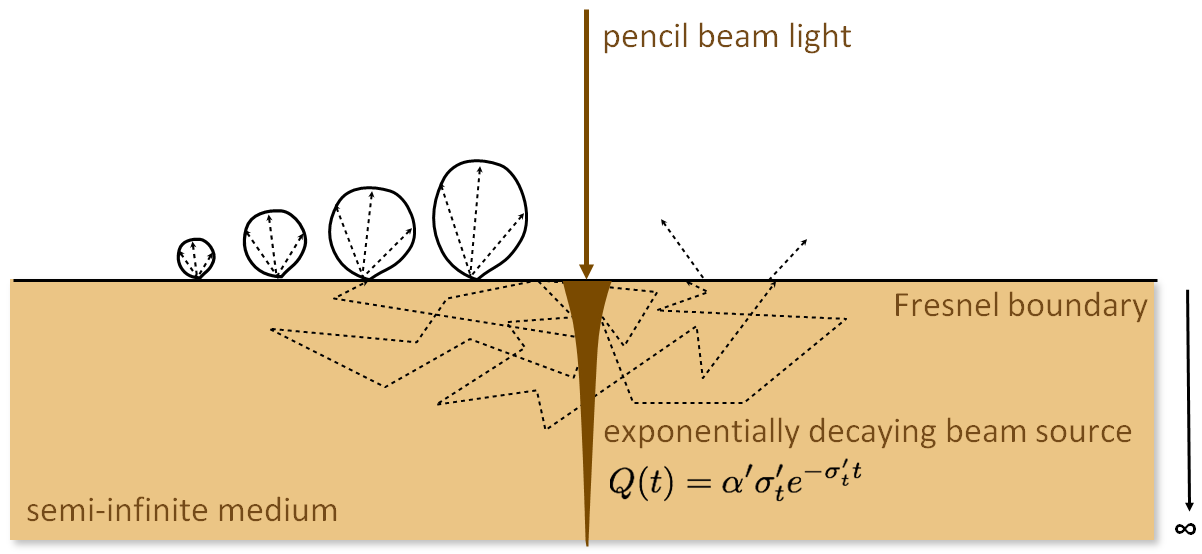
\includegraphics[width=\textwidth]{imgs/schemes/searchlight_disney}
    \caption{Schematic view of the searchlight experiment. To change.}
    \label{fig:searchlight_scheme}
\end{figure}

The term is: \gls{infiniteslab}

\section{Donner's Empirical BSSRDF}
This strange \gls{BSSRDF}
\comment{I like the reasoning here}
Donner et al. in \cite{Donner:2009:EBM} claim that the sum of single scattering
simulation and diffusion approximation (isotropic multiple scattering) does not
able to capture materials with relatively large suspended particles (such as
orange juice or milk). Because of the significant amount of light in scattered
duirng to low-oreder scattering events and high absorbtion.
These materials exhibit significant absorption of the light as it propagates
through the material, so much of the energy is scattered back into
the environment near the point of incidence. This light exits in areas and
directions outside of the single scattering regime, but not in the high-order
multiple scattering regime.

In the same paper !(probably) there is a statement:
mean-free path gives the scale of the response for a given material. For two
materials that differ only by $l$, we can predict the response of the second
material by scaling the response of the first material by the ratio of their
mean-free-paths.

In this work they use Monte Carlo particle tracing to tabulate an empirical
BSSRDF model for a flat surface on a homogeneous semi-infinite volume.
They represented the hemispherical distribution of light leaving the surface,
depending on the angle of the incident light, the relative position of the
exitant light, and the physical parameters (volume albedo, mean free path
length, phase function, and index of refraction). Their tables took months to
compute and contain around 250MB of data.

\section{Scattering in the thin objecs}
Diffuse transmission BTDF as a fast approximation of subsurface scattering in
thin materials.
Many real world objects like sheets of paper or foliege of the trees has strong
scattering component. There is a simple and inexpensive technique to approximate
scattering in such objects by using the Lambertian BTDF.

\ldots
